\section{SEDflow} \label{sec:sedflow}
In this work we apply ANPE to SED modeling of galaxy spectra. 
tl;dr of intro 

% section explaining specific SED set up 
\subsection{SED Modeling: PROVABGS} \label{sec:provabgs}
To model SEDs, we use the state-of-the-art stellar population synthesis (SPS)
model of the PROVABGS~(\chedit{Hahn~\etal~2022}). 
With SPS modeling, we model the SED of a galaxy a as a composite of stellar
populations defined by stellar evolution theory (in the form of isochrones,
stellar spectral libraries, and an initial mass function) and its star
formation and chemical enrichment histories (SFH and ZH), attenuated by
dust~\citep[see][for a review]{conroy2013}. 
The PROVABGS model, in particular, utilizes a non-parametric SFH with a
starburst, a non-parametric ZH that varies with time, and a flexible dust
attenuation prescription.

% highlight advantages of provabgs 
The SFH has two components: one based on non-negative matrix factorization
(NMF) bases and the other, a starburst component.
The SFH contribution from the NMF component is a linear combination of four NMF
SFH basis functions, that are derived from performing NMF~\citep{lee1999,
cichocki2009, fevotte2011}
on smoothed SFHs of simulated galaxiese of the Illustris cosmological
hydrodyanmic simulations~\citep{vogelsberger2014, genel2014, nelson2015}.
The NMF SFH prescription provides a compact and flexible representation of the
SFH, assuming that the SFHs of Illustris galaxies resemble the SFHs of real
galaxies. 
To add stochasticity to the SFH, we include a second star burst component that
consists of a single stellar population (SSP). 

The ZH is similar defined using two NMF bases dervied from Illustris ZHs. 
Most SPS models assume constant metallicity over
time~\citep[\emph{e.g.}][]{carnall2017, leja2019}; however, this assumption can
significantly bias inferred galaxy properties~\citep{thorne2021}. 
Instead by using the NMF prescription, we can flexibly model a range of
different ZHs with only two extra parameters.  
The stellar evolution theory is based on Flexible Stellar Population
Synthesis~\citep[FSPS;][]{conroy2009, conroy2010c} with the MIST
isochrones~\citep{paxton2011, paxton2013, paxton2015, choi2016, dotter2016},  
the \cite{chabrier2003} initial mass function (IMF), and a combination of the
MILES~\citep{sanchez-blazquez2006} and BaSeL~\citep{lejeune1997, lejeune1998,
westera2002} libraries.
The SFH and ZH are binned into 43 logarithmically-space time bin and SSPs are
evalulated at each time bin using FSPS. 
The SSPs are summed up to get the unattenuated galaxy SED. 

Finally, PROVABGS attenuates the light from the composite stellar population
using the two component \cite{charlot2000} dust attenuation model with
diffuse-dust (ISM) and birth cloud (BC) components. 
All SSPs are attenuated by the diffuse dust using the \cite{kriek2013}
attenuation curve.
Then, the BC component provides extra dust attenuation on SSPs younger than 100
Myr with young stars that are embedded in modecular clouds and HII regions. 
In total the PROVABGS SED model has 12 free parameters: stellar mass ($M_*$),
six SFH parameters ($\beta_1, \beta_2, \beta_3, \beta_4, t_{\rm burst}, f_{\rm
burst}$), two ZH parameters ($\gamma_1, \gamma2$), and three dust attenuation
parameters ($\tau_{\rm BC}, \tau_{\rm ISM}, n_{\rm dust}$). 
Each PROVABGS model evaluation takes \chedit{X} seconds. 

\subsection{Training Data} \label{sec:training}
In this section, we describe how to we construct the training data using our
SED model.
First, we sample $N_{\rm train}$ SED model parameters from a prior: $\theta'\sim p(\theta)$. 
We use the same priors as \chedit{Hahn \etal~(2022)}: uniform priors over $M_*,
t_{\rm burst}, f_{\rm burst}, \gamma_1, \gamma2, \tau_{\rm BC}, \tau_{\rm ISM},
n_{\rm dust}$ and Dirichlet prior over $\beta_1, \beta_2, \beta_3, \beta_4$. 
The Dirichlet prior is chosen for the normalization of the NMF SFH while the
rest are chosen to span an extensive range of galaxy SEDs. 

For each of the sampled SED parameters, we construct mock observables. 
In this work, our observables are optical photometry of the NASA-Sloan Atlas
(Section~\ref{sec:obs}).
We first input $\theta'$ into the SED model to construct galaxy SEDs: 
$F(\lambda;\theta')$. 
Afterwards, we convolve the SEDs with optical broadband filters, $R_X$ to
generate noiseless photometric fluxes:
\begin{equation}
    f_X(\theta') = \int F(\lambda;\theta') \, R_X(\lambda) \, {\rm d}\lambda
\end{equation}

Next, to generate synthetic photometry, we must apply a realistic noise model.


\begin{itemize}
    \item noise model 
\end{itemize}

\subsection{Training ANPE} \label{sec:anpe}
description of the ANPE training
\begin{itemize}
    \item architecture
    \item validation 
\end{itemize}

\begin{figure}
\begin{center}
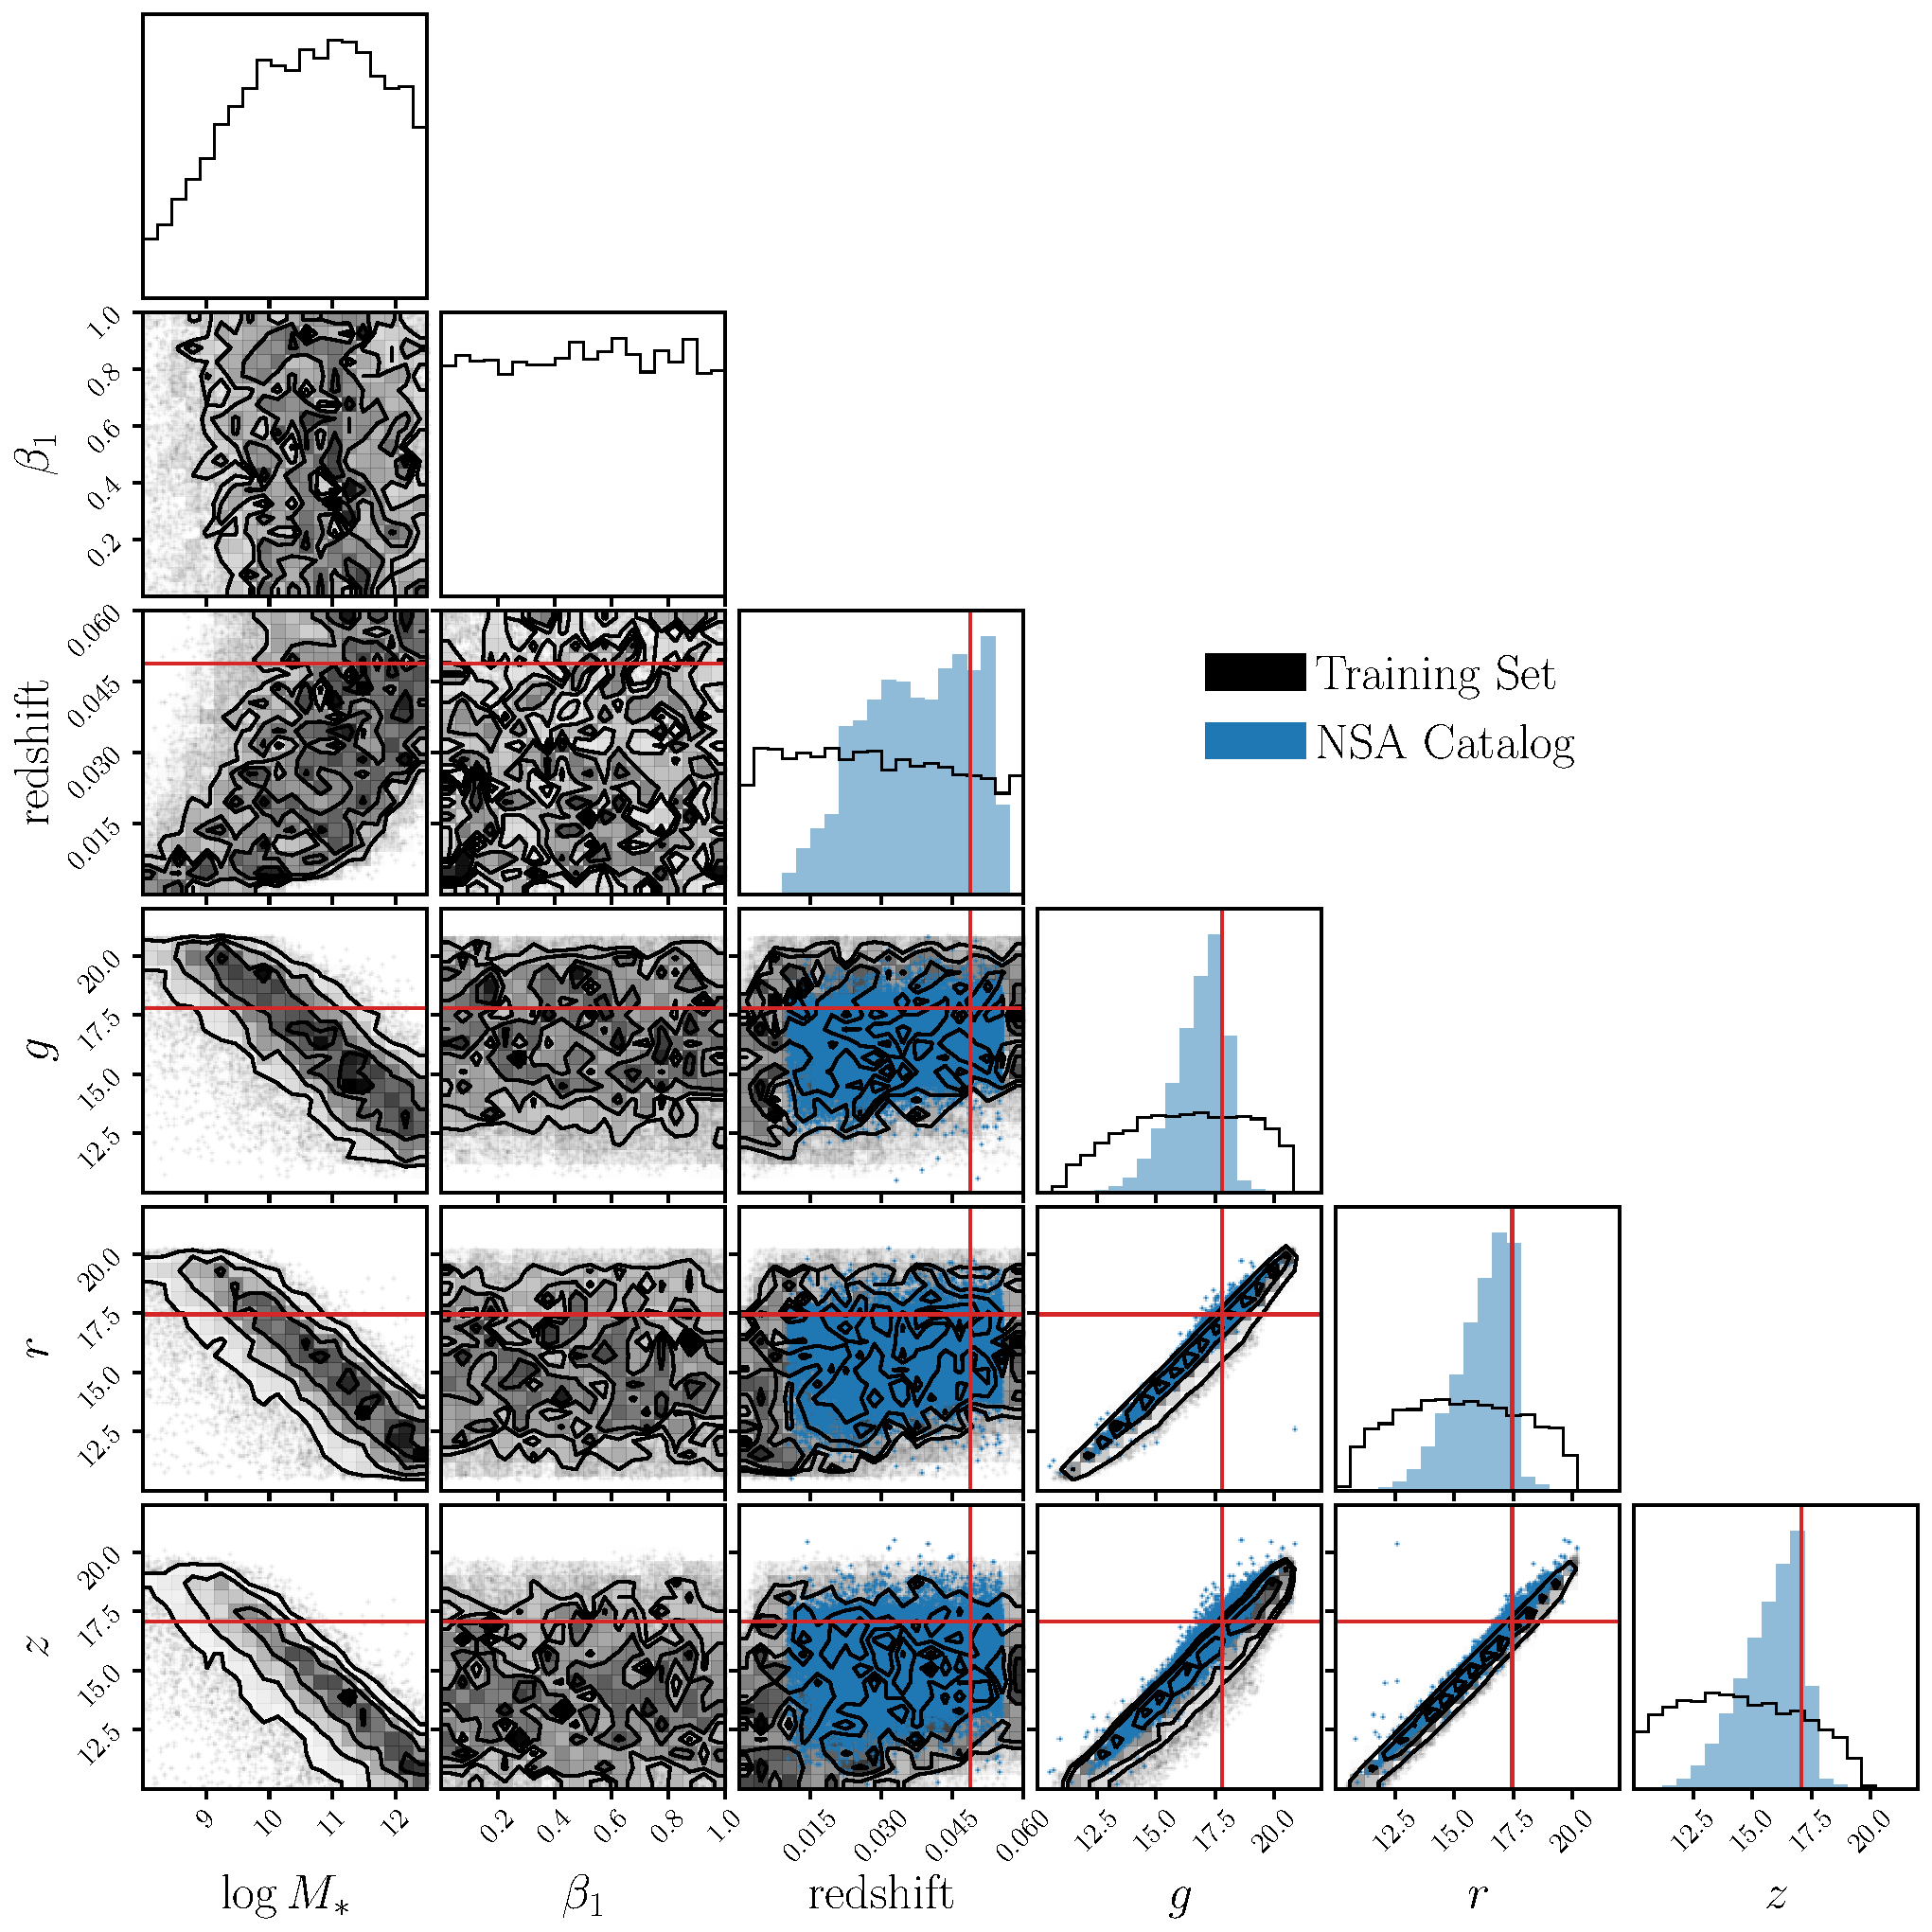
\includegraphics[width=0.9\textwidth]{figs/training.pdf}
    \caption{\label{fig:data}
    Joint distribution of SED model parameters ($\log M_*$, $\beta_1$,
    redshift) and photometric magnitudes ($g$, $r$, $z$) for our training set.
    The training set was constructed by sampling parameter values from the
    prior (Table~\ref{tab:prior}), constructing SEDs using a theoretical SPS
    model, and applying our noise model. 
    For details, we refer readers to Section~\ref{sec:sbi_sed}.
    For comparison, we present the distribution of magnitudes for galaxies in
    the NSA catalog (blue). 
    \emph{The training set fully encompasses the observations, thus, our 
    {\sc SEDflow} method can be used to infer the posterior for all NSA
    galaxies}.
    }
\end{center}
\end{figure}
